\documentclass[aspectratio=169]{beamer}

% Theme: Metropolis (clean, modern, minimal)
\usetheme{metropolis}

% Custom Colors for a professional look
\definecolor{primaryColor}{RGB}{0, 102, 128}  % Teal
\setbeamercolor{frametitle}{bg=primaryColor, fg=white}
\setbeamercolor{title separator}{fg=primaryColor}
\setbeamercolor{progress bar}{fg=primaryColor}
\setbeamercolor{alerted text}{fg=primaryColor}

% Packages
\usepackage{graphicx}
\usepackage{booktabs}
\usepackage{adjustbox}
\usepackage{caption}
\usepackage{hyperref}

% Graphics Path
\graphicspath{{figures/}}

% Title Information
\title[Internship Defense]{Industrial Training Defense}
\subtitle{Full-Stack Web Development at Tanbel Inc.}
\author{Jubaer Al Mamun \scriptsize\textit{(Software Engineer, Tanbel Inc., Dec 2023 - Present)} \\ ID: 221902013}
\institute{Department of CSE \\ Green University of Bangladesh}
\date{Fall 2025}

% Set Figure and Table Numbering
\setbeamertemplate{caption}[numbered]

\begin{document}

% Slide 1: Title Slide with Logos
{\setbeamertemplate{headline}{
    \leavevmode
    \hbox{
        \begin{beamercolorbox}[wd=0.5\paperwidth,ht=1.2cm,left]{}
            \hspace{0.5cm}
\includegraphics[height=1cm]{GUBLogoNew.png}
        \end{beamercolorbox}
        \begin{beamercolorbox}[wd=0.5\paperwidth,ht=1.2cm,right]{}
            \hfill
\includegraphics[height=0.7cm]{wecycle_logo.png}\hspace{0.5cm}
        \end{beamercolorbox}
    }
}
\begin{frame}
    \titlepage
\end{frame}
}

% Slide 2: Acknowledgment - Supervisors & Board Members
\begin{frame}{Acknowledgment}
    % Supervisors Section
    \textbf{\Large Supervisors}
    \vspace{0.3cm}
    
    \begin{columns}[T]
        \column{0.5\textwidth}
        \centering
        \textbf{Academic Supervisor}\\
        \vspace{0.1cm}
        Md. Parvez Hossain\\
        \textit{Lecturer, Dept. of CSE}\\
        Green University of Bangladesh

        \column{0.5\textwidth}
        \centering
        \textbf{Industrial Supervisor}\\
        \vspace{0.1cm}
        MD Tanvir Ahmed\\
        \textit{Product Manager}\\
        Tanbel Inc. (WeCycle)
    \end{columns}

    \vspace{0.6cm}

    % Board Members Section
    \textbf{\Large Board Members}
    \vspace{0.3cm}
    
    \begin{columns}[T]
        \column{0.5\textwidth}
        \centering
        Fatema Akter\\
        \textit{Lecturer, Dept. of CSE}\\
        Green University of Bangladesh

        \column{0.5\textwidth}
        \centering
        Mayeesha Farjana\\
        \textit{Lecturer, Dept. of CSE}\\
        Green University of Bangladesh
    \end{columns}
\end{frame}

% Slide 3: Table of Contents
\begin{frame}{Contents}
    \tableofcontents
\end{frame}

% Section 1: Organization Overview
\section{Organization Overview}
\begin{frame}{Organization Overview}
    \begin{columns}
        \column{0.55\textwidth}
        \textbf{Tanbel Inc. (WeCycle / ArrayQ) [1], [2]}
        \begin{itemize}
            \item \textbf{Industry:} Junk Removal SaaS.
            \item \textbf{Location:} United States (Remote Team).
            \item \textbf{Structure:} Flat, Agile Startup.
            \item \textbf{Products:}
            \begin{itemize}
                \item \textbf{WeCycle (B2C):} On-demand junk removal.
                \item \textbf{ArrayQ (B2B):} CRM dashboard for haulers.
            \end{itemize}
            \item \textbf{Mission:} Automate waste management \& promote sustainability.
        \end{itemize}

        \column{0.45\textwidth}
        \begin{figure}
            \centering
            
\includegraphics[width=0.5\textwidth]{wecycle_logo.png}
            \caption{WeCycle Logo}
        \end{figure}
        \begin{figure}
            \centering
            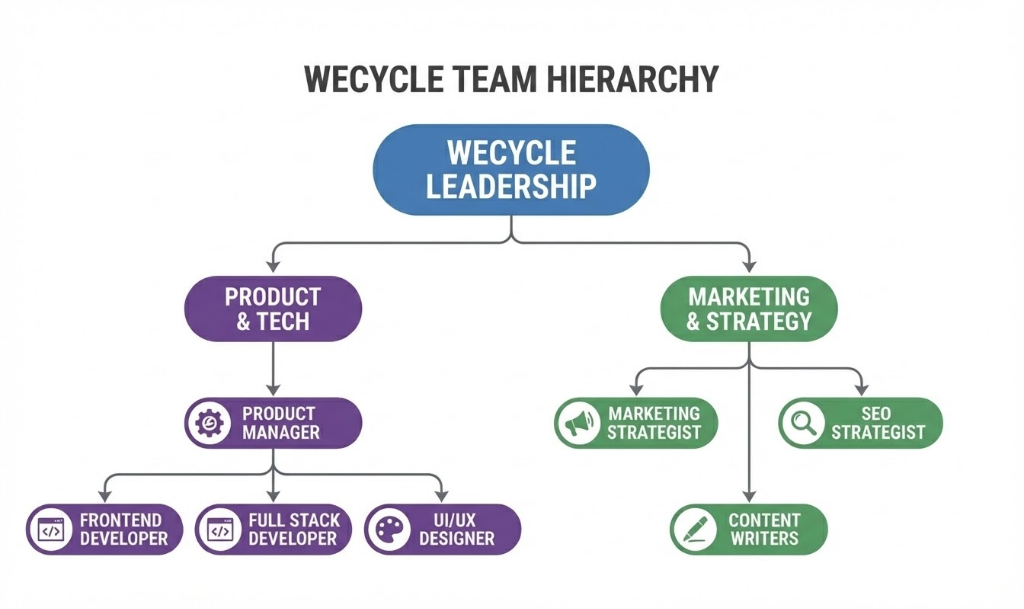
\includegraphics[width=0.85\textwidth]{wecycle_org_structure.png}
            \caption{Organizational Structure}
        \end{figure}
    \end{columns}
\end{frame}

% Section 2: Specific Details on Training Activities
\section{Specific Details on Training Activities}
\begin{frame}{Specific Details on Training Activities}
    \textbf{Role:} Full-Stack Web Developer | \textbf{Duration:} 8 Weeks (Oct - Dec 2025)

    \vspace{0.2cm}

    \begin{columns}
        \column{0.5\textwidth}
        \textbf{Key Projects:}
        \begin{itemize}
            \item \textbf{ArrayQ Launch:} Developed B2B landing page with multi-tenant branding.
            \item \textbf{AI Chatbot:} Deployed Dockerized chatbot with Nginx \& SSL.
            \item \textbf{Stripe Connect:} Automated hauler payouts.
            \item \textbf{UI Migration:} Migrated 10+ pages from Ant Design to Shadcn/ui [6].
        \end{itemize}

        \column{0.5\textwidth}
        \begin{figure}
            \centering
            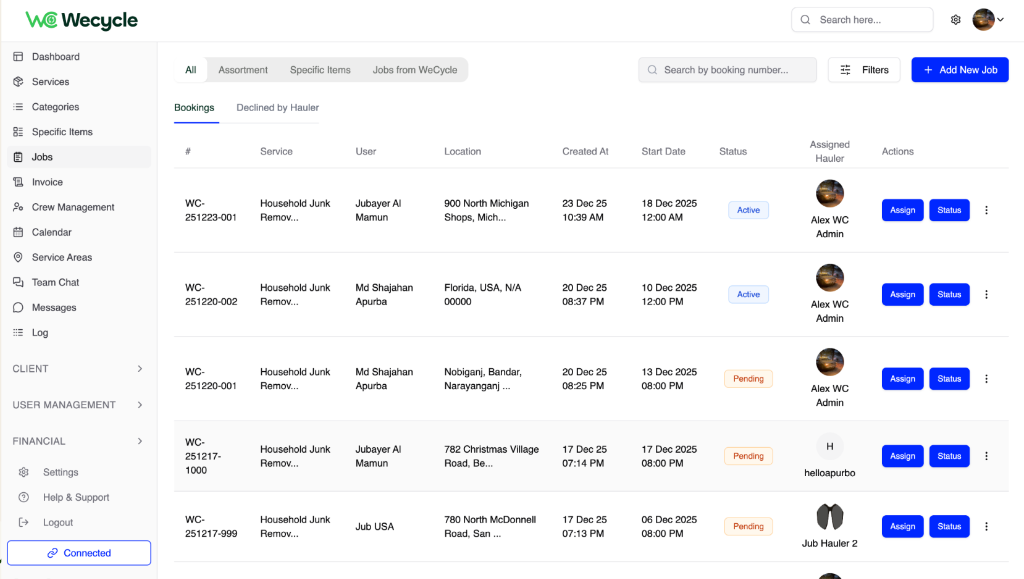
\includegraphics[width=0.95\textwidth]{dashboard_jobs.png}
            \caption{Jobs Management Dashboard}
        \end{figure}
    \end{columns}
\end{frame}

% Section 3: Acquired Skills
\section{Acquired Skills During Industrial Training}
\begin{frame}{Acquired Skills During Industrial Training}
    \begin{columns}
        \column{0.5\textwidth}
        \textbf{Technical Skills:}
        \begin{itemize}
            \item \textbf{Frontend:} Next.js 14 [3], React [4], TypeScript, Tailwind CSS [5].
            \item \textbf{Backend:} Node.js, Express, REST APIs.
            \item \textbf{Mobile:} Capacitor.js, React Native.
            \item \textbf{DevOps:} Docker, Nginx, GitHub Actions CI/CD.
        \end{itemize}

        \vspace{0.1cm}
        \textbf{Professional Skills:}
        \begin{itemize}
            \item Agile/Scrum Workflow (Jira).
            \item Remote Collaboration \& Standups.
            \item Code Review \& Version Control.
        \end{itemize}

        \column{0.5\textwidth}
        \begin{figure}
            \centering
            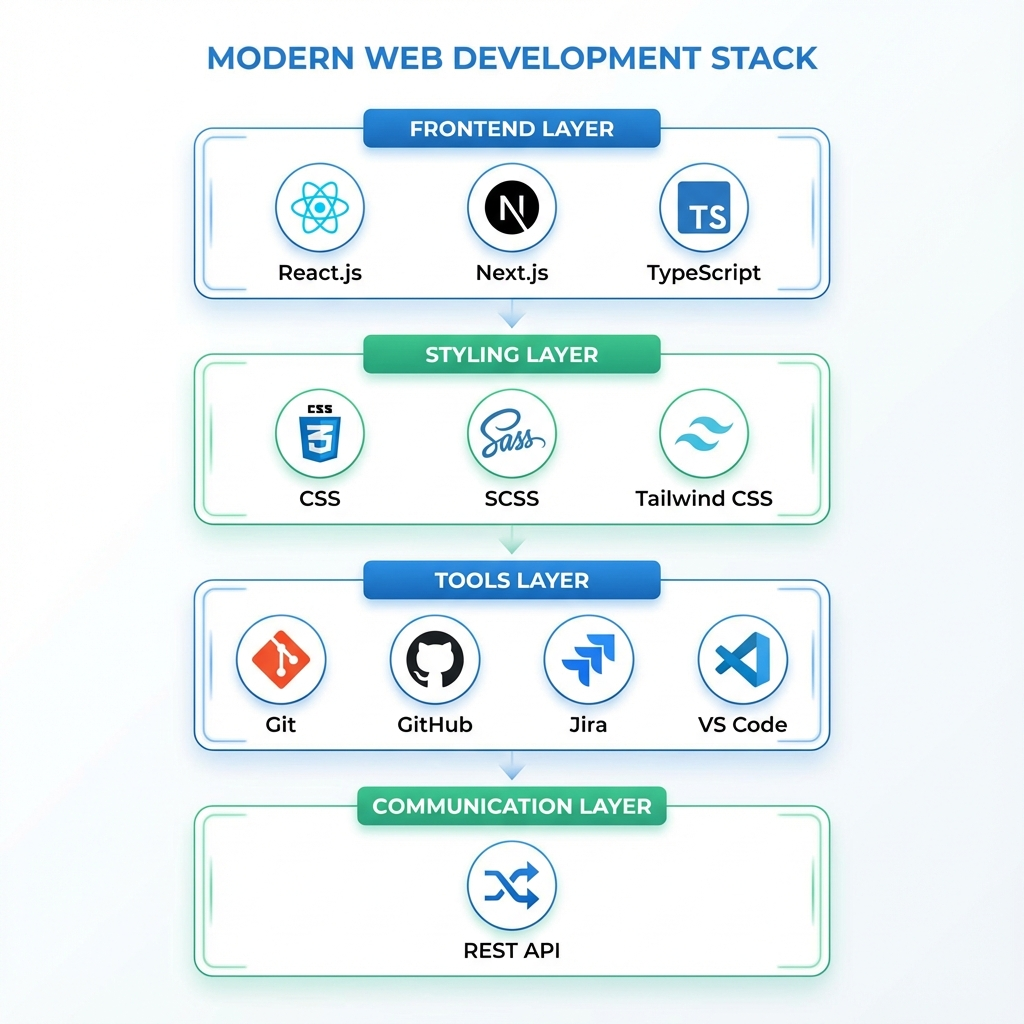
\includegraphics[width=0.9\textwidth]{tech_stack_diagram.png}
            \caption{Technology Stack Overview}
        \end{figure}
    \end{columns}
\end{frame}

% Section 4: PO-Skill Mapping
\section{PO-Skill Mapping}
\begin{frame}{PO-Skill Mapping}
    \begin{table}
        \centering
        \caption{Program Outcome (PO) Fulfillment}
        \resizebox{0.95\textwidth}{!}{
        \begin{tabular}{l l l}
            \toprule
            \textbf{Program Outcome} & \textbf{Skill Applied} & \textbf{Evidence} \\
            \midrule
            PO1: Engineering Knowledge & Algorithmic Logic & Complex lead filtering systems. \\
            PO2: Problem Analysis & Debugging & Diagnosed 15+ iPad-specific UI bugs. \\
            PO3: Design/Development & Scalable Architecture & Job Details \& Blog page design. \\
            PO5: Modern Tools & Industry Stack & Next.js [3], Docker, Jira, CI/CD. \\
            PO9: Teamwork & Collaboration & Daily standups, peer code reviews. \\
            PO12: Lifelong Learning & Self-Learning & Google Places API, advanced TS. \\
            \bottomrule
        \end{tabular}
        }
    \end{table}
\end{frame}

% Section 5: SDG-Goal Mapping
\section{SDG--Goal Mapping}
\begin{frame}{SDG--Goal Mapping}
    \begin{table}
        \centering
        \caption{SDG Goal Alignment}
        \resizebox{0.9\textwidth}{!}{
        \begin{tabular}{l p{9cm} l}
            \toprule
            \textbf{SDG Goal} & \textbf{Contribution} & \textbf{Fulfillment} \\
            \midrule
            SDG 8: Decent Work & Empowered gig-economy haulers with better tools. & Fully Fulfilled \\
            SDG 9: Industry \& Innovation & Built digital infrastructure for waste management. & Fully Fulfilled \\
            SDG 11: Sustainable Cities & Enabled rapid urban junk removal via software. & Fully Fulfilled \\
            SDG 12: Responsible Consumption & Promoted proper disposal \& recycling. & Fully Fulfilled \\
            \bottomrule
        \end{tabular}
        }
    \end{table}
\end{frame}

% Section 6: Conclusion
\section{Conclusion}
\begin{frame}{Conclusion}
    \centering
    \Large \textbf{``I didn't just learn. I shipped.''}

    \vspace{0.5cm}

    \normalsize
    \begin{itemize}
        \item Transitioned from academic projects to \textbf{production engineering}.
        \item Resolved \textbf{70+ Jira tickets} and delivered critical features.
        \item Gained confidence in navigating complexities of a \textbf{remote startup}.
        \item Ready to contribute effectively to the \textbf{software industry}.
    \end{itemize}
\end{frame}

% References Slide
\begin{frame}{References}
    \footnotesize
    \begin{enumerate}
        \item WeCycle, ``WeCycle: Eco-Friendly Junk Removal and Recycling Services,'' 2024. [Online]. Available: \url{https://getwecycle.com/}
        \item WeCycle, ``WeCycle Hauler: Professional Junk Hauling Services,'' 2024. [Online]. Available: \url{https://getwecycle.com/hauler}
        \item Vercel Inc., ``Next.js Documentation,'' 2024. [Online]. Available: \url{https://nextjs.org/docs}
        \item Meta Platforms, Inc., ``React Learn: Getting Started with React,'' 2024. [Online]. Available: \url{https://react.dev/learn}
        \item Tailwind Labs Inc., ``Tailwind CSS Documentation,'' 2024. [Online]. Available: \url{https://tailwindcss.com/docs}
        \item shadcn, ``shadcn/ui: Beautifully Designed Components,'' 2024. [Online]. Available: \url{https://ui.shadcn.com/docs}
    \end{enumerate}
\end{frame}

% Thank You Slide
\begin{frame}
    \centering
    \vspace{2cm}
    {\Huge \textbf{Thank You!}}
    
    \vspace{1cm}
    {\Large \textit{Questions?}}
    
    \vspace{1.5cm}
    \normalsize
    Jubaer Al Mamun\\
    ID: 221902013\\
    Department of CSE, Green University of Bangladesh
\end{frame}

\end{document}
